\section{Skyscraper}

\begin{frame}
	\frametitle{Skyscraper}
	\begin{block}{Description}<1->
		\begin{itemize}
			\item Quadratic field with side length $n$
			\item Place differently sized skyscraper on field, height $\in[1,n]$
		\end{itemize}
	\end{block}
	\begin{block}{Constraints}<2->
		\begin{itemize}
			\item No two skyscraper with the same height in each row/column
			\item Number of visible skyscrapers from the side
		\end{itemize}
	\end{block}
\end{frame}

\begin{frame}
	\frametitle{Example}
	\begin{figure}
		\centering
		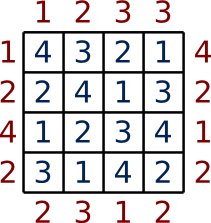
\includegraphics[height=6cm]{images/skyscraper.png}
	\end{figure}
\end{frame}

\begin{frame}
	\frametitle{Encoding}
	\begin{block}{State space}<1->
		\begin{itemize}
			\item Skyscraper variables: $v_{x,y}^{h}$ with $x,y,h\in[1,n]$
			\item Semantic: $v_{x,y}^{h} \equiv 1 \Leftrightarrow$ Skyscraper with height $h$ on field $x,y$
		\end{itemize}
	\end{block}
	\begin{itemize}
		\item<2-> On every field there has to be at least one skyscraper
		\begin{displaymath}
			\bigwedge_{x,y} \bigvee_{h} v_{x,y}^h
		\end{displaymath}
	\end{itemize}
\end{frame}

\begin{frame}
	\frametitle{Encoding cont.}
	\begin{itemize}
		\item On every field there has to be at most one skyscraper
		\begin{displaymath}
			\bigwedge_{x,y} \bigwedge_{h\not=h^{\prime}} \neg(v_{x,y}^{h} \wedge v_{x,y}^{h^{\prime}})
		\end{displaymath}
		\item<2-> No two equally high skyscraper in each row/column
		\begin{displaymath}
			\bigwedge_{h,c} \bigwedge_{k\not=l} \neg(v_{c,k}^{h} \wedge v_{c,l}^{h}) \wedge \neg (v_{k,c}^{h} \wedge v_{l,c}^{h})
		\end{displaymath}
	\end{itemize}
\end{frame}

\begin{frame}
	\frametitle{Constraint encoding}
	\begin{itemize}
		\item Counting function $numS$ and memory function $maxS$
		\begin{displaymath}
			maxS_{d}(\pmb x) = 
			\begin{cases}
				height(\pmb x)+1 & height(\pmb x) \ge mS_{d}(\pmb x + \pmb e_{d})\\
				maxS_{d}(\pmb x + \pmb e_{d}) &\text{if not}
			\end{cases}
		\end{displaymath}
		\begin{displaymath}
			numS_{d}(\pmb x) =
			\begin{cases}
				numS_{d}(\pmb x - \pmb e_{d}) + 1 & height(\pmb x) \ge maxS_{d}(\pmb x)\\
				numS_{d}(\pmb x - \pmb e_{d}) &\text{if not}
			\end{cases}
		\end{displaymath}
		\item $d\in \{North, East, South, West\}$
		\item $\pmb e_{North} = (-1,0)^T, \pmb e_{East} = (0,1)^T, \pmb e_{South} = (1,0)^T,\pmb e_{West} = (0,-1)^T$
	\end{itemize}
\end{frame}

\begin{frame}
	\frametitle{Constraint encoding cont.}
	\begin{columns}
		\begin{column}{6cm}
			\begin{itemize}
				\item Constraint $c$ adds clause $numS_{d}(\pmb x) = c$ to formula
				\item <2-> Polynomial reduction in side length of field $O(n^3)$
			\end{itemize}
		\end{column}
		\begin{column}{5cm}<2->
			\begin{figure}
				\centering
				
\includegraphics[width=5cm]{images/win.jpg}
			\end{figure}
		\end{column}
	\end{columns}
\end{frame}

\begin{frame}
	\centering
	\hfill \Large Live demonstration \hfill\hfill
\end{frame}
